\clearpage
\section{\name{} Annotation Tool (Beta)}
\label{appendix:annotation_tool}
This section documents the \name{} annotation and validation interface, a beta-stage prototype designed to facilitate systematic literature reviews (SLRs) through the integration of LLM-assisted information extraction and expert-led verification. 

\begin{figure}[h]
    \centering
    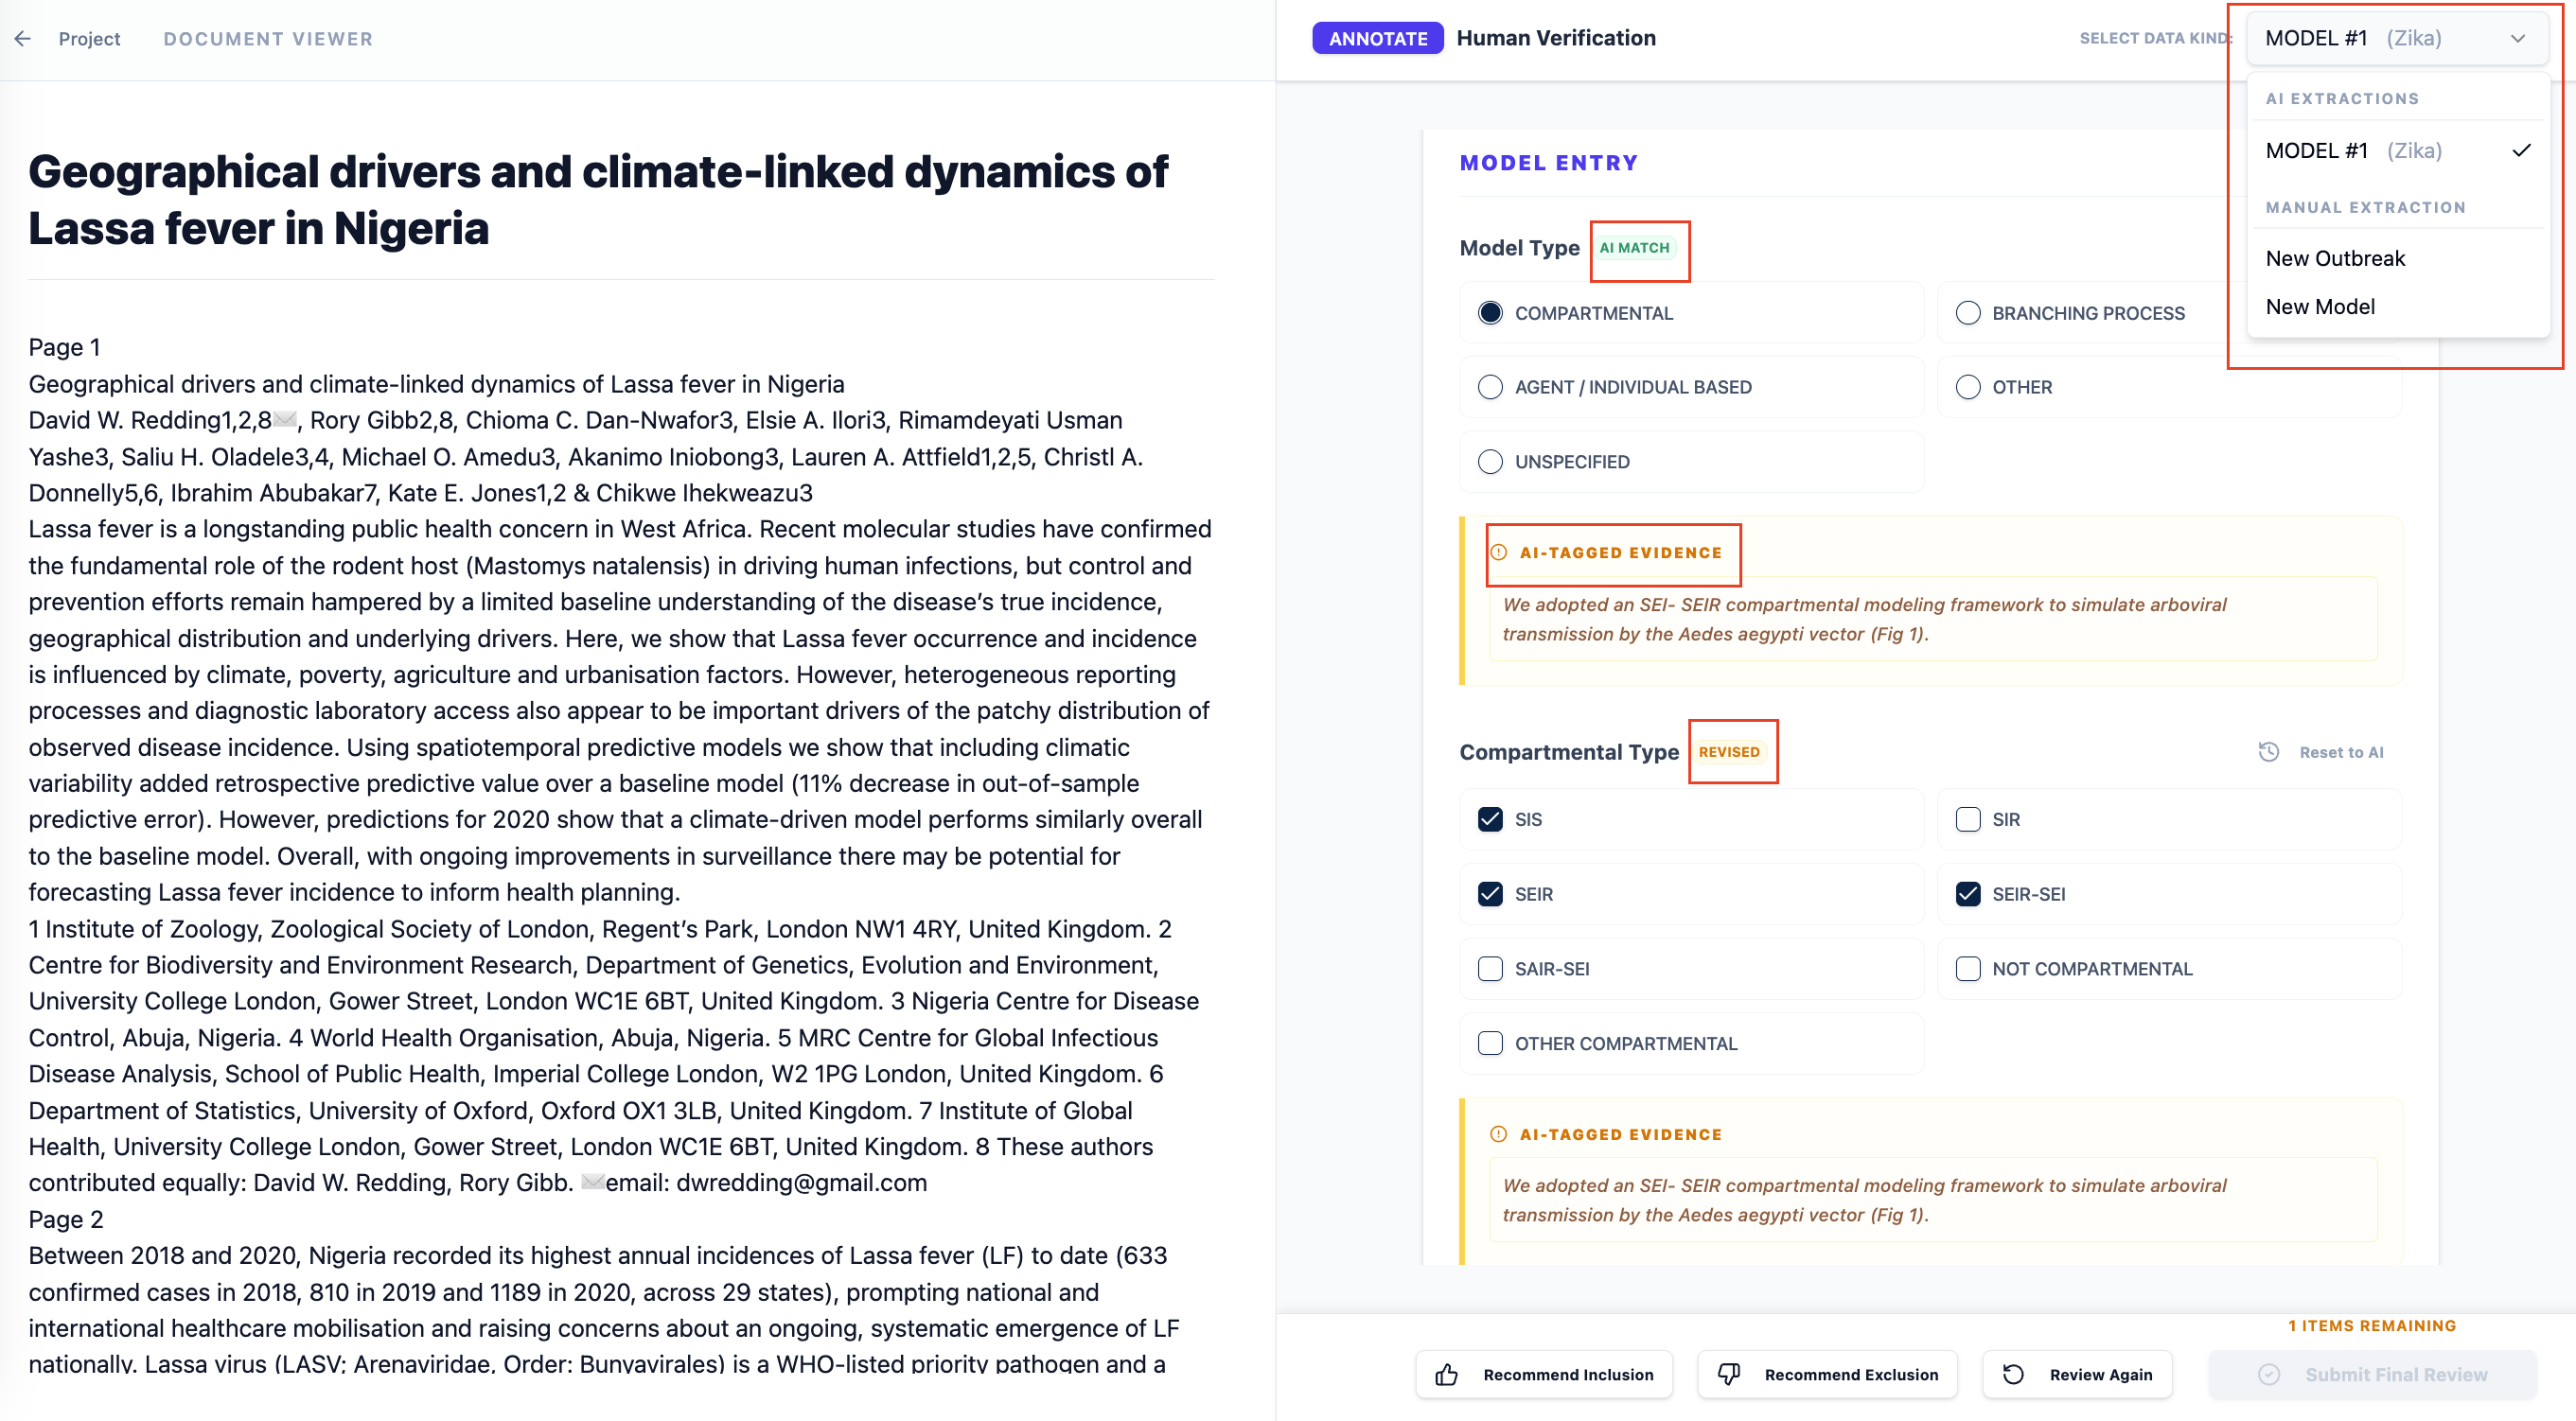
\includegraphics[width=0.95\textwidth]{figures/annotation/ann_tool_main.png}
    \caption{\textbf{The \name{} extraction and validation tool interface.} The dual-pane view presents the source document (\textbf{left}) alongside structured extraction fields (\textbf{right}). AI-predicted entries are pre-filled and accompanied by highlighted, AI-tagged evidence excerpts from the manuscript. Reviewers can accept, revise, or reject individual fields, with validation status indicators (e.g. ``AI Match'' or ``Revised'') reflecting whether human intervention was required.}
    \label{fig:ann_main}
\end{figure}

\subsection{System Architecture and Core Functionality}
The \name{} annotation tool provides an interactive environment for technical validation of automated information extractions. The system utilises data gathered by LLMs equipped with structured tool-calling to identify and parse epidemiological parameters, transmission models, and outbreak characteristics. To ensure transparency and auditability, the tool implements a provenance layer that maps every extracted value to specific textual excerpts (AI-tagged evidence) within the source article.

\subsection{User Interface Design}
The interface is optimised for high-throughput expert review via a dual-panel architecture:
\vspace{-10pt}
\begin{itemize}[leftmargin=*, itemsep=-3pt]
    \item \textit{Document Viewer (Left Panel):} Provides the original article text or rendered PDF, ensuring reviewers can verify the context of any extracted data point without context switching.
    \item \textit{Verification Interface (Right Panel):} Displays a form-based view of pre-filled fields generated by the \name{} pipeline. The extraction schema is dynamic, adapting based on the identified content type, such as compartmental model variables or spatio-temporal outbreak data.
\end{itemize}

\subsection{Human-in-the-Loop Validation}
The framework enforces a human-in-the-loop (HITL) protocol where automated extractions are audited by subject matter experts before being finalised for evidence synthesis. Within the interface, reviewers perform the following actions:
\vspace{-10pt}
\begin{itemize}[leftmargin=*, itemsep=-3pt]
    \item \textit{Verify:} Confirm the accuracy of the AI-extracted value and its linked evidence.
    \item \textit{Modify:} Correct extraction errors or refine data granularity; modified entries are flagged as ``Revised'' to facilitate system error analysis.
    \item \textit{Reject:} Entirely dismiss false positive extractions that do not meet inclusion criteria.
\end{itemize}

\subsection{Current Status and Field Testing}
The tool is currently in a beta development phase, with pilot testing conducted by epidemiologists focusing on WHO priority pathogens. While the current pilot utilises epidemiology-specific schemas, the architecture is designed to be domain-agnostic and can be adapted through schema reconfiguration and expert consultation.

Planned field testing is aligned with the Pathogen Epidemiology Review Group (PERG) workflow for remaining priority pathogens. This testing will utilise standardised extraction schemas for parameter, model, and outbreak data, and specifically target  systematic reviews for CCHF virus and Rift Valley fever virus.

\begin{figure}[t]
    \centering
    \begin{minipage}[b]{0.48\textwidth}
        \centering
        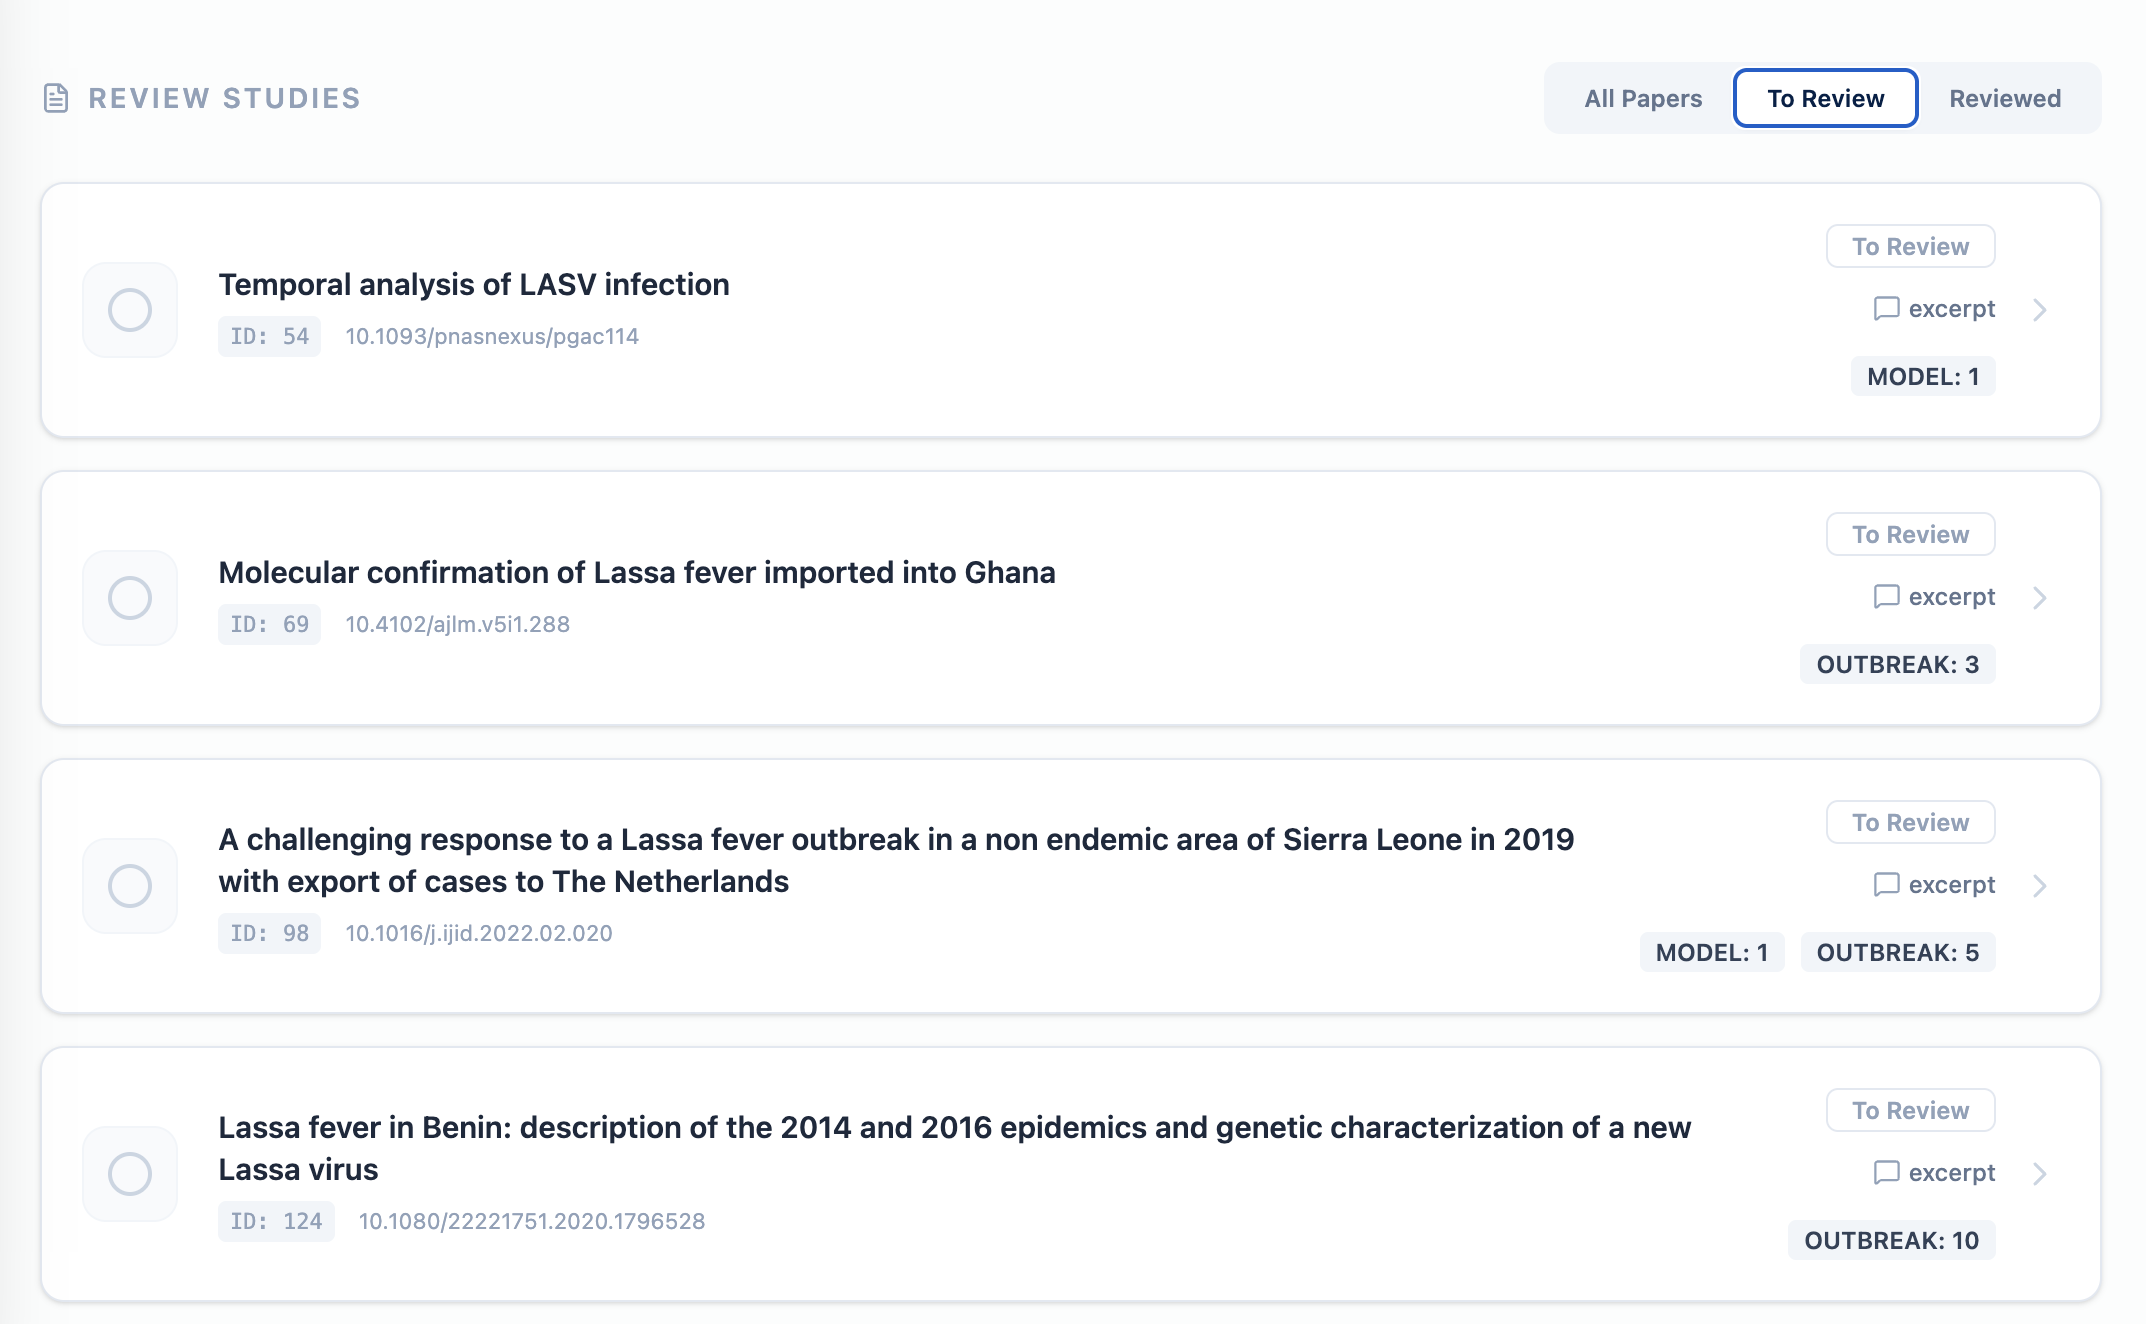
\includegraphics[height=5.7cm,keepaspectratio]{figures/annotation/ann_tool_multiple_papers_to_review.png}
        \caption*{(a) Tool Management Dashboard}
    \end{minipage}\hfill
    \begin{minipage}[b]{0.48\textwidth}
        \centering
        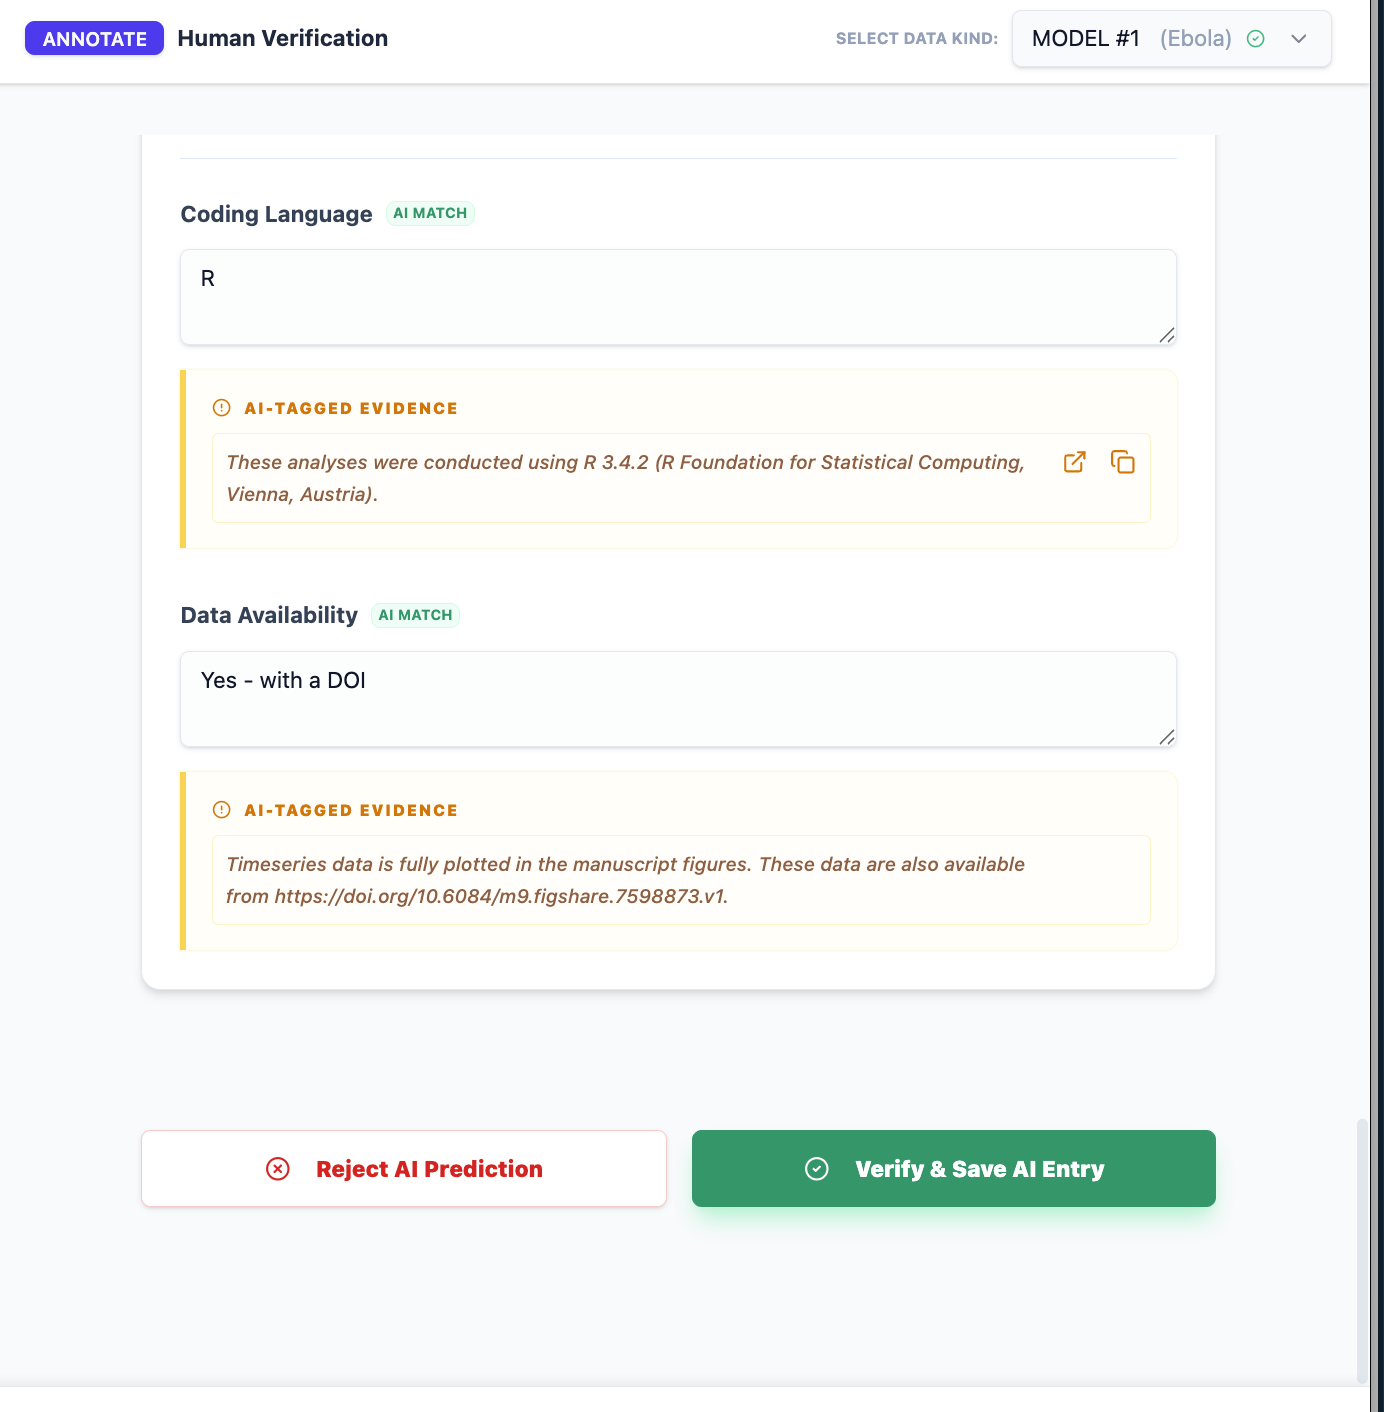
\includegraphics[height=5.2cm,keepaspectratio]{figures/annotation/ann_tool_verify_and_submit.png}
        \caption*{(b) Verification and Submission}
    \end{minipage}
    \caption{\textbf{Review management and submission tracking interfaces.} (a) The study review list displays papers awaiting expert validation, along with associated model and outbreak counts and direct links to extracted excerpts. (b) The verification view presents finalised AI-assisted extractions, enabling reviewers to explicitly reject predictions or verify and save corrected entries, which are then recorded for downstream quality control and system evaluation.}
    \label{fig:ann_logistics}
\end{figure}

\subsection{Transparency and Reproducibility}
By maintaining a persistent link between the structured database and the source text, \name{} ensures that synthesised reports can be fully disaggregated. This audit trail is critical for scientific reproducibility, allowing researchers to trace every reported parameter, model and outbreak back to its exact location in the primary literature.